\documentclass{standalone}
\usepackage{tikz}
\usepackage{amssymb,amsmath,amsthm}
\usepackage{graphicx}
\usepackage{caption}
\usetikzlibrary{shadows,matrix} % Shadows for nodes
\usetikzlibrary{positioning}
\usetikzlibrary{arrows.meta}
\begin{document}
\tikzset{darkstyle/.style={circle,draw,fill=gray!40}}
\centering
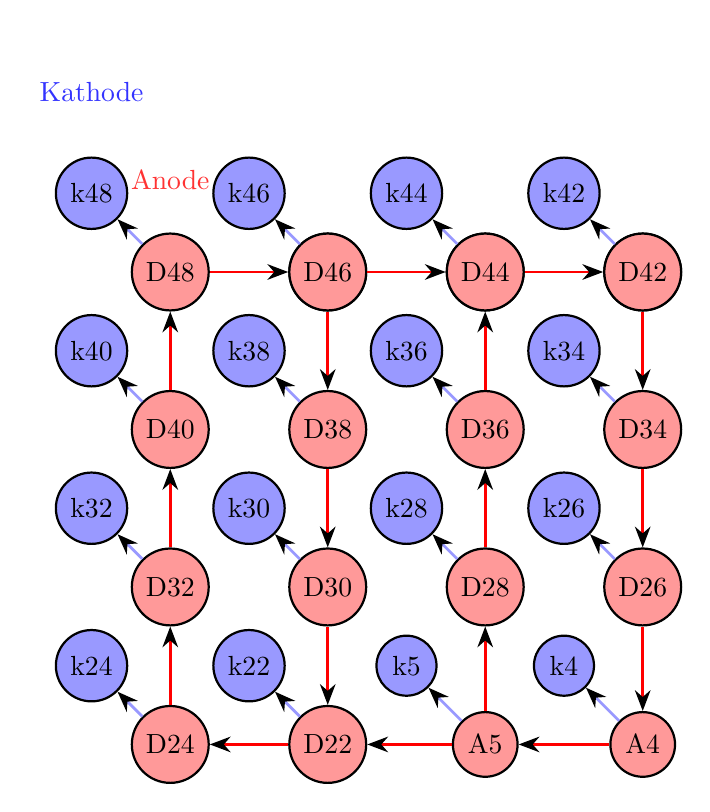
\begin{tikzpicture}
\begin{scope}[every node/.style={circle,thick,draw,fill=red!40,level distance=200mm,}]
    \node [label=above:\rotatebox{0.0}{\textcolor{red!80}{Anode}}] (D48) at (0,0) {D48};
    \node (D46) at (2,0) {D46};
    \node (D44) at (4,0) {D44};
    \node (D42) at (6,0) {D42};
    
    \node  (D46) at (2,0) {D46};
    \node  (D44) at (4,0) {D44};
    \node  (D42) at (6,0) {D42};
    
    \node (D40) at (0,-2) {D40};
    \node (D38) at (2,-2)  {D38};
    \node (D36) at (4,-2) {D36};
    \node (D34) at (6,-2) {D34};
    
    \node (D32) at (0,-4) {D32};
    \node (D30) at (2,-4)  {D30};
    \node (D28) at (4,-4) {D28};
    \node (D26) at (6,-4) {D26};
    
    \node (D24) at (0,-6) {D24};
    \node (D22) at (2,-6)  {D22};
    \node (A5) at (4,-6) {A5};
    \node (A4) at (6,-6) {A4};
    
\end{scope}

\begin{scope}[>={Stealth[black]},
              every node/.style={fill=gray!40,circle,thick},
              every edge/.style={draw=red,very thick}]
     \draw [color=red!100,->,line width=1] (A4) -- (A5);
     \draw [color=red!100,->,line width=1] (A5) -- (D22);
     \draw [color=red!100,->,line width=1] (D22) -- (D24);
     \draw [color=red!100,->,line width=1] (D24) -- (D32);
     \draw [color=red!100,->,line width=1] (D32) -- (D40);
     \draw [color=red!100,->,line width=1] (D40) -- (D48);
     
     \draw [color=red!100,->,line width=1] (D48) -- (D46);
     
     \draw [color=red!100,->,line width=1] (D46) -- (D38);
     \draw [color=red!100,->,line width=1] (D38) -- (D30);
     \draw [color=red!100,->,line width=1] (D30) -- (D22);
     
     \draw [color=red!100,->,line width=1] (D46) -- (D44);
     \draw [color=red!100,<-,line width=1] (D44) -- (D36);
     \draw [color=red!100,<-,line width=1] (D36) -- (D28);
     \draw [color=red!100,<-,line width=1] (D28) -- (A5);
     
     \draw [color=red!100,->,line width=1] (D44) -- (D42);
     \draw [color=red!100,->,line width=1] (D42) -- (D34);
     \draw [color=red!100,->,line width=1] (D34) -- (D26);
     \draw [color=red!100,->,line width=1] (D26) -- (A4);
   
\end{scope}
\begin{scope}[every node/.style={circle,thick,draw,fill=blue!40,level distance=200mm,}]
    \node [label=above:\rotatebox{0.0}{\textcolor{blue!80}{Kathode}}]  (k48) at (-1,1) {k48};
    \node (k40) at (-1,-1) {k40};
    \node (k32) at (-1,-3) {k32};
    \node (k24) at (-1,-5) {k24};  
    
    \node (k46) at (1,1) {k46};
    \node (k38) at (1,-1) {k38};
    \node (k30) at (1,-3) {k30};
    \node (k22) at (1,-5) {k22};
    
    \node (k44) at (3,1) {k44};
    \node (k36) at (3,-1) {k36};
    \node (k28) at (3,-3) {k28};
    \node (k5) at (3,-5) {k5}; 
    
    \node (k42) at (5,1) {k42};
    \node (k34) at (5,-1) {k34};
    \node (k26) at (5,-3) {k26};
    \node (k4) at (5,-5) {k4}; 
    
\end{scope}

\begin{scope}[>={Stealth[black]},
              every node/.style={fill=gray!40,circle,thick},
              every edge/.style={draw=red,very thick}]

     \draw [color=blue!40,->,line width=1] (D48) -- (k48);
     \draw [color=blue!40,->,line width=1] (D40) -- (k40);
     \draw [color=blue!40,->,line width=1] (D32) -- (k32);
     \draw [color=blue!40,->,line width=1] (D24) -- (k24);

     \draw [color=blue!40,->,line width=1] (D46) -- (k46);
     \draw [color=blue!40,->,line width=1] (D38) -- (k38);
     \draw [color=blue!40,->,line width=1] (D30) -- (k30);
     \draw [color=blue!40,->,line width=1] (D22) -- (k22);     

     \draw [color=blue!40,->,line width=1] (D44) -- (k44);
     \draw [color=blue!40,->,line width=1] (D36) -- (k36);
     \draw [color=blue!40,->,line width=1] (D28) -- (k28);
     \draw [color=blue!40,->,line width=1] (A5) -- (k5); 

     \draw [color=blue!40,->,line width=1] (D42) -- (k42);
     \draw [color=blue!40,->,line width=1] (D34) -- (k34);
     \draw [color=blue!40,->,line width=1] (D26) -- (k26);
     \draw [color=blue!40,->,line width=1] (A4) -- (k4); 
                  
\end{scope}
\end{tikzpicture}
\end{document}